\documentclass[10pt]{article}
\usepackage[margin=0.82in]{geometry}
\usepackage{graphicx,booktabs,xcolor,microtype,parskip}
\definecolor{navy}{HTML}{18334B}\definecolor{teal}{HTML}{176B87}
\usepackage[colorlinks=true,linkcolor=teal,urlcolor=teal]{hyperref}
\title{\vspace{-2em}\color{navy}\bfseries IDM-Viz localization audit\\[-.2em]\large 30-seed held-out synthetic evaluation}
\author{Phase 3 empirical addendum}\date{17 November 2026}
\begin{document}\maketitle\vspace{-1em}
\section*{Question and protocol}
We separately tested (i) dependence-pair identification and (ii) mapping frozen clusters to five known generating regions. All cluster-to-region maps were fitted using the historical training rows only. Pair thresholds used historical reference and calibration inputs only. We then applied the frozen mappings and thresholds to 30 evaluation seeds, each with 96 consecutive 500-row batches. Monitoring labels and region IDs were evaluator-only. Confidence intervals resample seeds (2,000 bootstrap replicates); batches are not treated as independent.
\section*{Dependence pair}
During the designed marginal-preserving correlation change, the linear-task detector alarmed on 1.000\ of active batches (seed-bootstrap 95\% CI: 1.000--1.000); its top pair matched the intervention pair in 1.000\ of batches (CI: 1.000--1.000). This favorable result applies to one specified intervention law. On the stationary control, the empirically calibrated detector alarmed at approximately its intended 5\% operating rate. It does not establish localization under arbitrary dependence shifts.
\begin{center}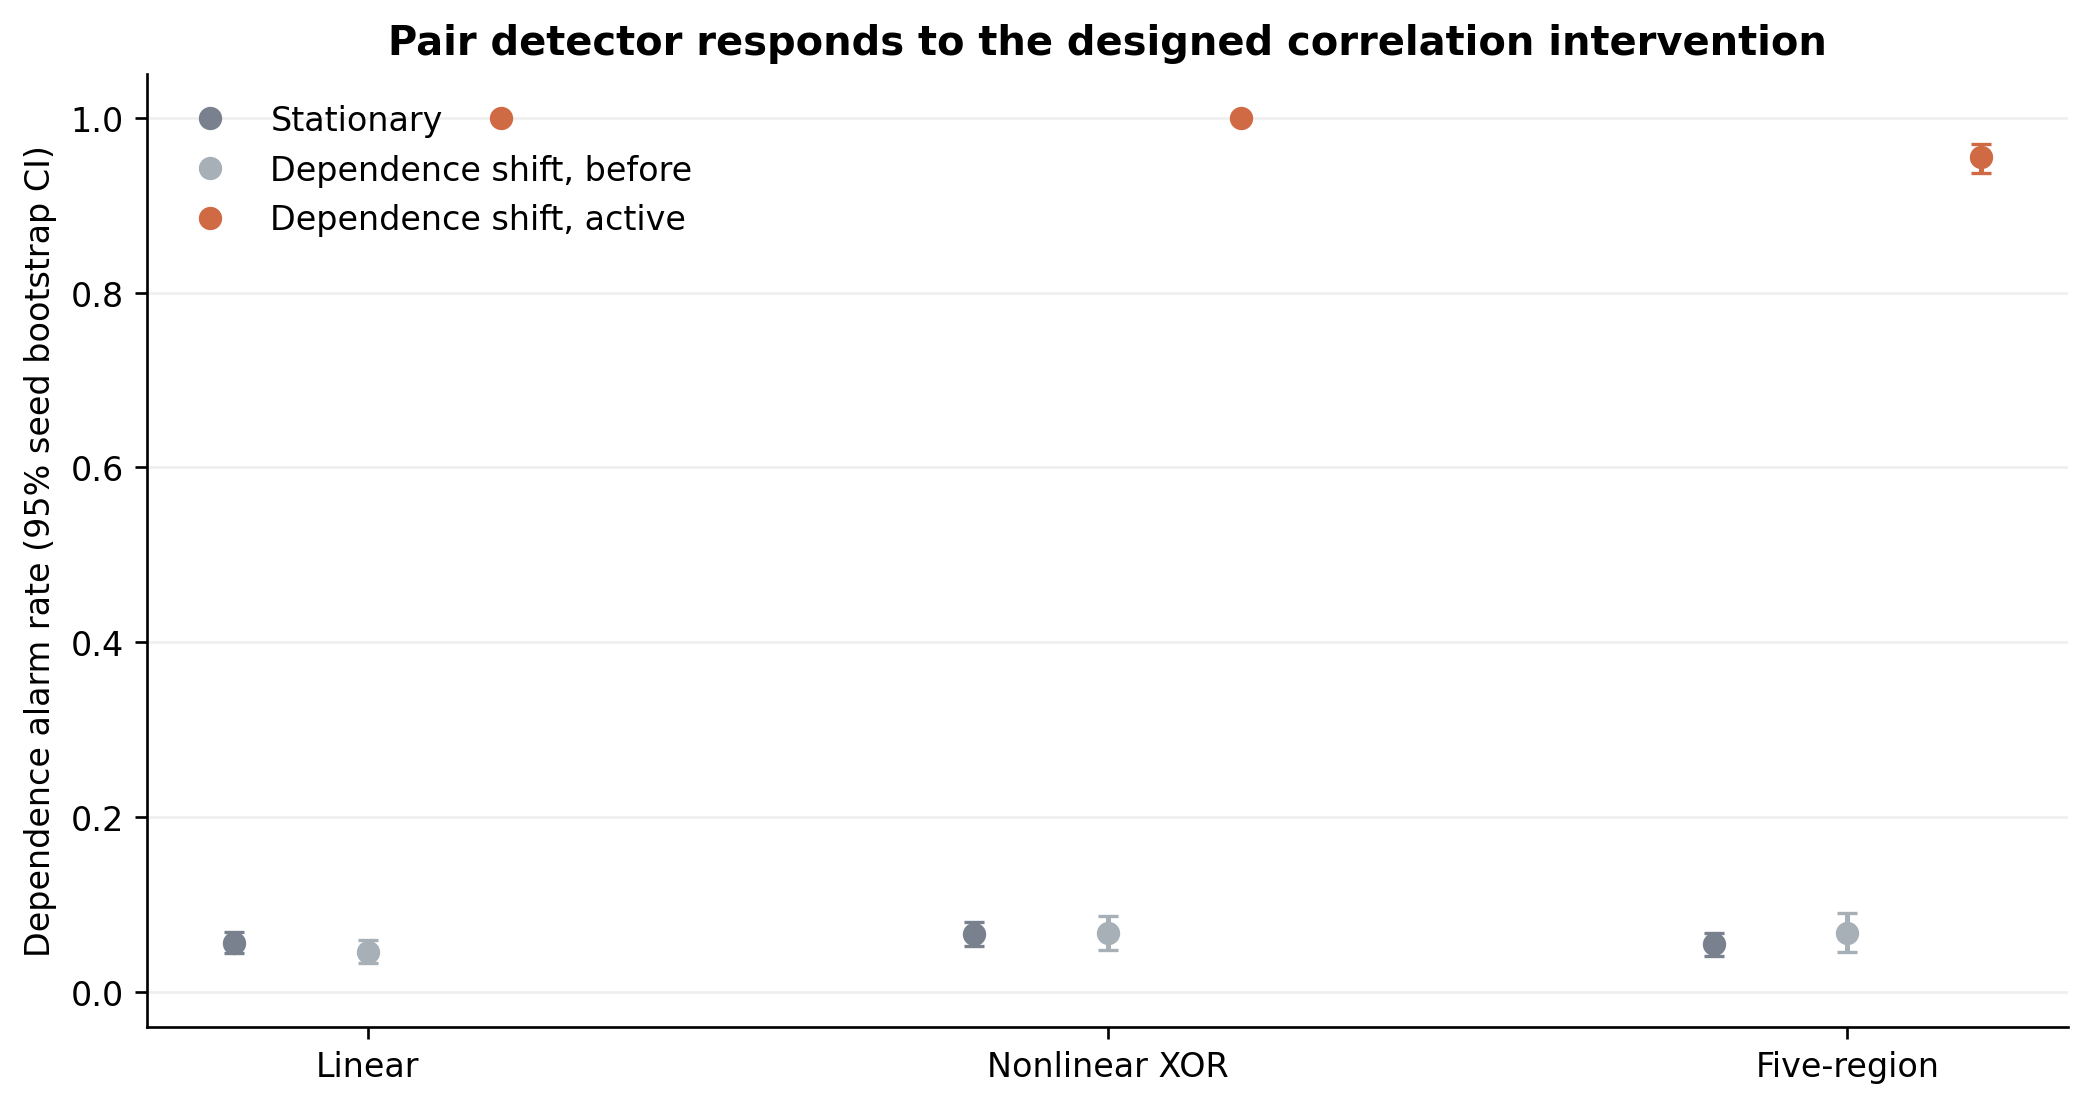
\includegraphics[width=.95\linewidth]{dependence_detection.png}\end{center}
\section*{Generating-region assignment}
The five-cluster model achieved seed-mean adjusted Rand index 0.088 (CI: 0.080--0.097). During the abrupt local reversal, its recall for the truly intervened region was 0.216 (CI: 0.207--0.225). Other cluster counts have similar weaknesses and may leave regions unmapped. The selected cluster count is not a reliable substitute for region identity; the visualization should expose uncertainty and occupancy rather than label these clusters as known regions.
\begin{center}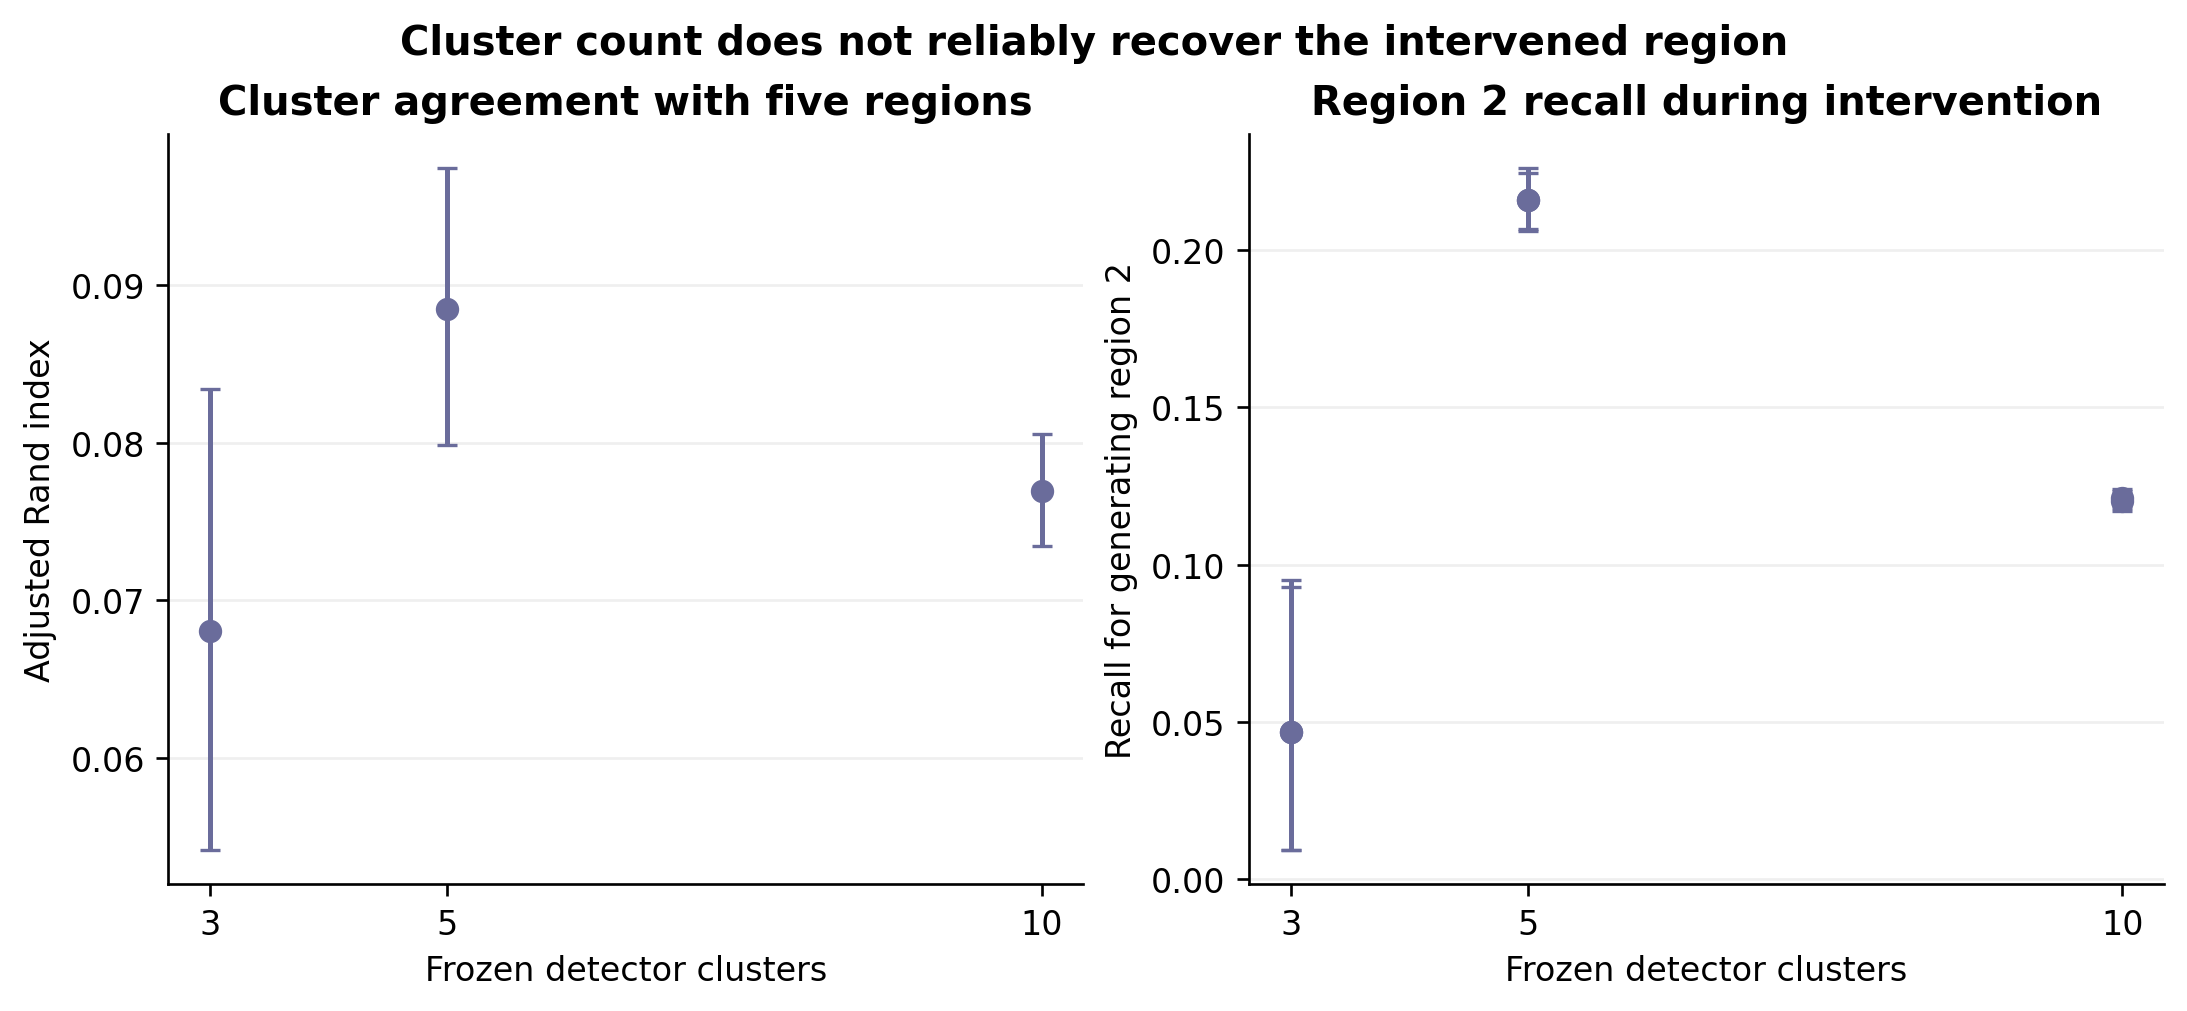
\includegraphics[width=.95\linewidth]{region_localization.png}\end{center}
\section*{Interpretation}
The audit closes a measurement gap by providing target-specific localization metrics, and it finds that regional localization is weak. The pair result is a targeted synthetic positive control, not broad validation. No causal responsibility, operational benefit, or analyst decision improvement follows from these measurements. Full raw seed and batch rows, mappings, thresholds and checksums are in the accompanying result directory. The current complete project test suite reports 176 passing tests; this report is an exploratory post-hoc diagnostic on the locked evaluation seed bank and was not used to tune thresholds or models.
\end{document}
